%% Based on a TeXnicCenter-Template by Gyorgy SZEIDL.
%%%%%%%%%%%%%%%%%%%%%%%%%%%%%%%%%%%%%%%%%%%%%%%%%%%%%%%%%%%%%

%------------------------------------------------------------
%
\documentclass{amsart}
%
%----------------------------------------------------------
% This is a sample document for the AMS LaTeX Article Class
% Class options
%        -- Point size:  8pt, 9pt, 10pt (default), 11pt, 12pt
%        -- Paper size:  letterpaper(default), a4paper
%        -- Orientation: portrait(default), landscape
%        -- Print size:  oneside, twoside(default)
%        -- Quality:     final(default), draft
%        -- Title page:  notitlepage, titlepage(default)
%        -- Start chapter on left:
%                        openright(default), openany
%        -- Columns:     onecolumn(default), twocolumn
%        -- Omit extra math features:
%                        nomath
%        -- AMSfonts:    noamsfonts
%        -- PSAMSFonts  (fewer AMSfonts sizes):
%                        psamsfonts
%        -- Equation numbering:
%                        leqno(default), reqno (equation numbers are on the right side)
%        -- Equation centering:
%                        centertags(default), tbtags
%        -- Displayed equations (centered is the default):
%                        fleqn (equations start at the same distance from the right side)
%        -- Electronic journal:
%                        e-only
%------------------------------------------------------------
% For instance the command
%          \documentclass[a4paper,12pt,reqno]{amsart}
% ensures that the paper size is a4, fonts are typeset at the size 12p
% and the equation numbers are on the right side
%
\usepackage{amsmath}%
\usepackage{amsfonts}%
\usepackage{amssymb}%
\usepackage{graphicx}
%------------------------------------------------------------
% Theorem like environments
%
\newtheorem{theorem}{Theorem}
\theoremstyle{plain}
\newtheorem{acknowledgement}{Acknowledgement}
\newtheorem{algorithm}{Algorithm}
\newtheorem{axiom}{Axiom}
\newtheorem{case}{Case}
\newtheorem{claim}{Claim}
\newtheorem{conclusion}{Conclusion}
\newtheorem{condition}{Condition}
\newtheorem{conjecture}{Conjecture}
\newtheorem{corollary}{Corollary}
\newtheorem{criterion}{Criterion}
\newtheorem{definition}{Definition}
\newtheorem{example}{Example}
\newtheorem{exercise}{Exercise}
\newtheorem{lemma}{Lemma}
\newtheorem{notation}{Notation}
\newtheorem{problem}{Problem}
\newtheorem{proposition}{Proposition}
\newtheorem{remark}{Remark}
\newtheorem{solution}{Solution}
\newtheorem{summary}{Summary}
\numberwithin{equation}{section}
%--------------------------------------------------------
\begin{document}
Description of the model\\
%\\
%1. Discrete network model\\
%\\
\\The scope of our model is to emulate they way that multiple cells or many body part of an organism connect with one an other, receive energy from the environment and distribute energy between them.
For these reasons we decided to formulate our model as a directed graph consisting of $N$ nodes, with the connections between nodes forming a network. Therefore, each node will correspond to a single cell or "body" part, and the directed connections between nodes correspond to the way the organism distributes the energy (osmosis, blood or sap transport, etc...).
\\This type of network model is usually represented with an $N \text{ x } N$ connectivity matrix, $A=(a_{ij})$ where \begin{displaymath}
   a_{ij}= \left\{
     \begin{array}{lr}
       1 : \text{if node }i \text{ connects to node } j &\\
       0 : \text{otherwise}&
     \end{array}
   \right.
\end{displaymath}
Each network configuration or \textit{topology} will therefore represent a different type of organism with its particular size (number of nodes $N$) and structure (matrix $A$). 
\\
%\\
 %a. Pump\\
\\For many organism one or several body parts, such as animals mouth or plants roots and leaves, are designed to acquire energy (food, water, light, nutrients, etc...) from their surrounding.
For our model we will assume that one node in the network receives a energy from the environment, and we will call this node the \textit{pump}. From the pump, the energy will then start to be transmitted along edges to all the other nodes in the network (main body). Heretofore, the pump will be labeled as node 1 in the connectivity matrix, and in diagrams as $P$, also note that while in our simplified model we are considering a single node as the source of energy, it is possible to easily extend this model to include the possibility of multiple pumps, however for this paper we will limit our discussion to one pump so that we can maintain our discussion as simple as possible.
\\
%\\
% b. Other nodes, d. Consumption of energy\\
%\\
\\
All nodes can receive a energy along each incoming edge and transmit energy along each outgoing edge, exactly as in the blood circulation nutrients are transported from one part of the body to the next. \\
Each node will also consume a constant amount of energy, $c$, therefore reducing the remaining energy to be transmitted to its outgoing connections to $E_{out}=E_{in}-c$. This correspond to the energy that is consumed to maintain a certain body part alive.
\\
%\\
% c. Connectivity rules\\
%\\
\\It is also necessary to give some restriction on the our networks. In fact for a living organism does not make sense to have a body part that cannot receive energy. If that would happen that body part should be effectively be considered as not part of the organism. Therefore, the network of nodes that we will consider are directed graphs that contains a directed path from the pump to any other node in the network, we will refer to this condition as \textit{pump-connectedness}. 
%\\
 %e. Cost of transport proportional to amount of transport\\
%\\
\\
Also, after the energy cost $C$ is applied, each node $i$ divides its remaining signal ($E_{out,i}$)(energy) into equal parts based on the total number of outward connections, $b_i$. We can think of this as the branching in a blood vessel. Moreover, during transport nutrients can degrade, be consumed by cell in the structure constituting the connection (epithelial cells in blood vessel) or leak back into the environment (water evaporating from the body) the amount of energy received by each of the $b_i$ successors should then be equal to a fraction, $p$, of the outgoing energy ($0\leq p\leq 1$): 
\begin{equation}
E_{in,j}=\frac{E_{out,i}\cdot p}{b_i}
\end{equation} 
%There are three cases to consider, $0<p<1: $ dissipative transport, the signal is reduced during transport; $p > 1: $ amplified transport, the signal increases during transport; and $p=1: $ neutral transport, the signal is unchanged during transport.\\
%\\
%\\
%2. Determining signal (energy) at each node\\
%\\
\\
The energy received by each node will then be given by the sum of the energies from inward connections. We will denote the energy that exits from node $i$ in the direction of node $j$ as $E_{ij}$. Therefore, given an initial environmental energy, $E_0$, we can calculate the energy entering each node $i$ using the formulas: 
\begin{equation}\label{eq:rec1}
E_i=\sum_{j=1}^N E_{ji}=\sum_{j=1}^N a_{ji}\frac{(E_j-c)p}{b_j}, \text{ For } i=2,\cdots, N 
\end{equation}
\begin{equation}\label{eq:rec2}
E_1=E_0+\sum_{j=1}^N E_{j1}=E_0+\sum_{j=1}^N a_{j1}\frac{(E_j-c)p}{b_j}
\end{equation}
where $E_i$ is the total incoming energy for node $i$ (Note: $E_i=E_{in, i}$ for node $i$) for $i=1,2,...,N$ and $E_0$ is the environmental (initial) energy that the organism gathers from the environment. [NOTE: May want to change notation to be more graph theoretical (i.e. $j\in V(G)$)]. An example of the use of \ref{eq:rec1} and \ref{eq:rec2} for a simple system is shown in figure 1[create reference]. 
\\
%\\
 %a. Given an energy that the pump receives, we can know the energy received by all other cells.\\
%\\
Note, that the previous formulas for a system of $N$ linear equations in $N+1$ unknowns ($E_i$ with $i=0,1,\ldots N$), and that this system is of maximum rank (Note: need proving). Therefore, if we know the  energy at one specific node $i$, using the previous linear system we can identify all the others, including the initial signal $E_0$ required for node $i$ to have that prescribed energy $E_i$. We will use this to identify important initial signal levels for the network.
\\
Simple examples (figure 1)\\
%\\
 %c. Critical energy - Knowing a point when a certain number of cells die, find the energy at the pump \\
%\\
	%i. Definition of critical energy for a specific node and its meaning\\
	\\
	The critical energy of the $k^{th}$ node $E^*_k$ is the lowest environmental energy at which the node can survive (i.e. $E_k \geq c$), meaning that the correspondent body part or cell is receiving enough energy. If the node does not receive enough energy the node dies. We can think of this as the organism being in a starvation condition and therefore starting to lose body mass (nodes).\\
	%\\
	%ii. How to compute\\
	%\\
To find this energy we take the previous linear system of $N$ equations and add the condition $E_k=c$ so that now we have $N$ equations in $N$ unknowns. Generally this system has a unique solution since the equations are linearly independent (needs prove?). Therefore, we can solve for the $E_i$ with $i=0,1,...,N$ and we have $E^*_k=E_0$.\\
%	\\
%	iii. Definition of ordinal critical energies and their meaning\\
%	\\

	Once we have a list of critical energies for all nodes, the first node to die will be the one with the largest critical energy, then the one with the second largest critical energy, and so on. Therefore, forming a list of critical energies in descending order, will correspond to have a list of death events, where every time the energy falls below a certain level one or multiple nodes will die, depending on the structure of network. The $r^{th}$ entry in this list will be called the $r^{th}$ critical energy and denoted $E^{*,r}$.\\
Note however then when calculating critical energies we should also take into consideration that nodes that receive less than $c$ amount of energies cannot transmit anymore to successive nodes, effectively changing the system to solve (this is a simple elimination of terms in the previous equations and can be easily implemented).
	\\
	\\
	\\
	\\
3. Special Networks\\
\\
Therefore, using our explicit formula we can solve the system and eventually write down the value of $E_0$ as a function of the other nodes energies, and by substitution obtain an explicit formula dependent on $c$ and $p$. However, for most topologies this process is very specific and knowing the explicit formula for one does not generally allows to express the same for an other topology.\\
Nevertheless, we can group topologies into ones that have common characteristic for which we can explicitly write the formula for critical energies. (Need to reformulate in terms of extendability: A sufficient condition to write the critical energies is for the topology to be acyclic). Some examples of such topologies are seen in figure 2 [reference figure. To include: Description of special topologies in caption, Topologies themselves, connectivity matrix, critical energies] 
[Followed by plots: .....].\\
For most of the paper from now on we will consider the first critical energy, corresponding to the condition to maintain all nodes alive, but we will also discuss how to find optimal structures for different critical energies (how not to lose more than a certain number of nodes) in the next section.
We will now illustrate in detail some of the groups of topologies previously mentioned.\\
We will start with the simplest \textit{star} and \textit{line}, and then move to slightly more complicated groups that we will call \textit{forks} and \textit{flares}. For these topologies finding the first node to die is relatively simple and therefore reconstructing an explicit formula for its critical energy its a simple reverse calculation. We will consider for this only the $1$st critical energy, since upon one death this topology still become topologies of one of the described types. For the rest of the paper we will simply use the term critical energy in relation to the $1$st one.\\
\\
 a. Line\\
\\
A line topology is one in which each node (except the last one, first to die) connects to one and only one other node and each node (except the first one, pump) is connected to one and only one other node (see fig.2). This topology maximizes the number of connections to reach the last node (first death), and is therefore the one (when the size of the network is fixed) that requires the highest energy to keep every node alive.\\
\\
 b. Star\\
\\
In a star topology the pump connects to all other nodes and these have no outgoing connections.
In this case all non-pump nodes will die at the same time, but the number of connections from pump to them is minimized to $1$ making this the topology with the lowest energy to keep everyone alive.\\
\\
 c. Importance of these motifs\\
\\
As we can see this two topologies, despite being the simplest, correspond to the two extreme points in terms of critical energies, being the best and the worst in terms of first critical energy.\\
Now we want to preserve some of The  of line and star studying hybrid topologies that are partially line-like and partially star-like.
\\
\\
\\

 d. Simple generalizations\\
\\To achieve this objective we will explore two possible approaches. In these groups we have topologies with only one node with multiple connections, but only at one of the two extremity of the our structure (an even further generalization with the bifurcation at any point on the longest line-path is presented in the supplementary material(?)).
\\
\\
  i. Fork\\
  A fork is a topology that extends as a line up to the $l$-th node and this node has $s$ connections one to each remaining node (see figure 2) (note that $l+s=n$ total number of nodes, and $l,s\geq 1$).
	\\
	\\
	ii. Flare (Stellar flare (re-name))\\
	A flare is a topology in which the pump has exactly $s$ outgoing connections and one of the branches formed this way has exactly length $l$ (not counting the pump) (note that $l+s=n$ total number of nodes, and $l,s\geq 1$).\\
	\\
	Note that for both flares and forks $l+s=n$ and these parameters can be used to indicate how close they are to be a line or a star, with $s=n-1$ and $l=1$ being a star, and $l=n-1$ and $s=1$ being a line.
	(more explanation in figure caption??) 
	\\
	\\
	\\
 e. Provide explicit formula of first critical energy\\
 In figure 2 we are summarizing these topologies and their explicit formulas for critical energy, while in figure 3 we are analyzing in details what happens to the critical energy for (?the forks and ?)flares when we fix $p,c,n$ and vary $s$. As we can see in this case depending on the environmental energy, both being close to a line or a star can be beneficial, but not being in an intermediate condition (more details in figure 3, parabola, net graphs, etc...)(should we include colormaps with only these special topologies for a certian size?).
\\
\\
\\
 f. Node to die is independent of c and p\\
 In all the previous topologies it is easy to find the first node to die and calculate its energy based on $E_0$, then imposing that this energy is exactly equal to $c$ we can find the corresponding critical energy. For the star and fork all the nodes after the bifurcation will have the same critical energy and will die first since they are the last to receive energy. while for line and flares only the final node with no outward connection will die at the first death event. Note that while stars reduce the required energy to keep everyone alive, they lose $n-1$ nodes all at once, while lines lose one node at a time. Flares and forks have instead an intermediate behavior, with the first losing one node at a time for the first $l-1$ nodes and then $s$ all at once, and the fork loses first $s$ nodes all at once and then $l-1$ nodes one at a time.
\\
\\
  i. only one path back to the pump\\
  This topologies are also particularly easy because for each node they have only one directed path connecting them to the pump, making the process of finding an explicit formula easier. However, the same process we used can be accomplished even with more paths (add example in the supp material?).\\
   One other important characteristic is the absence of loops that would make our explicit formula an infinite series. If we have loops it is still possible to write an explicit formula, but we need to be careful and check that our series converges (add figure to explain non converging case?). However, it is easy to see that in a biological settings with $0\leq p\leq 1$ and $c>0$ any eventual series due to loops will converge.\\
	\\
Simulations (should we call them simulations?)\\
\\
Now that we have defined the critical energies as \textit{metrics} to evaluate the success of topologies, and we have shown how simple topologies behave with respect to the first ordinal critical energy, we want to ask ourselves questions about this "metric" for some simple cases and then try to extract some information from more complicated one through simulations and analysis through statistical measures.\\
\\
First we want to show some interesting properties that can be seen when comparing some relatively simple topologies, then we will give a general rule to identify the "best" topology, and finally we will show results for a big number of topologies and some interesting statistical measure about their critical energies.\\
\\
4 topologies 5 nodes example / Coexistence and Conditional higher fitness\\\\
In figure 4 (colormap with 4 topologies) we are presenting four topologies all of size $n=5$ and we are plotting how many of them survive (do not lose nodes) for different values of $E_0$ and $p$.\\
 In  this simple cases we can still write down explicit formulas for the critical energy, and doing so verify that two of them have the same critical energy (bottom curve), and the other two have different critical energies with an intersection for $p=1/3$ (actual calculations shown in supp. material?).\\
Therefore, this simple example shows us that we can have networks with different topologies being equivalent in terms of critical energy, and different networks having critical energies for which one is conditionally better than the other.\\
We can think of the first phenomenon as the coexistence of two different species with the same fitness, following the idea that two species can adopt reach the same final result using different strategies. Instead the second one is like having two species whose fitness relative to each other changes depending on the efficiency in transporting energy (parameter $p$, common to both)), with one of the two structures to be preferred for less efficient species ($p\leq1/3$) and the other for more efficient species ($p\geq1/3$).\\
Moreover after observing this example is easy to imagine that more complicated situation could arise when considering more complex or a bigger number of networks. For instance, the coexistence of more than two network with same critical energy, two networks with multiple intersections, intersection in one point of more than two critical energies curves, etc... \\
However, trying to classify all the possible situation will require a lengthy exposition and is not the main purpose of our paper. \\
Instead we will now give a condition to be the "best" topology and relate this to the previous example.\\
\\
"Best" topology\\
\\
We have already established that considering $0\leq p\leq 1$ and $c>0$ the star topology is the one with the lowest $1st$ critical energy for any specific size $n$. Now we would like to state a general rule for the other ordinal critical energies.\\
Lets take for instance the $2nd$ critical energy for a network. We want to find the network of a fixed size $n$ whose second critical energy is the lowest possible. This critical energy is by definition the minimum energy before which we get a second node to die. Lets assume for now that 1st and 2nd critical energies are different. Therefore, we should consider a network of $n-1$ nodes with lowest $1st$ critical energy and add one node, in such a way that the added node will die before any of these $n-1$ nodes.\\ However, we already know that for networks of a certain size the topology with the lowest 1st critical energy is the star. Hence, our network is a star with $n-1$ nodes with an additional node connected only to one or more of the $n-2$ ramification from the center, and by construction the 2nd critical energy of this network is the same as the 1st critical energy of the star with $n-1$ nodes.\\
To complete our process, we finally consider the case in which 1st and 2nd critical energy are the same. If the best 2nd critical energy topology had this property, then the 2nd critical energy would be equal to the 1st critical energy and then will be higher or equal to the first critical energy for the star with $n$ nodes, but this is obviously bigger than the 1st critical energy of the star with $n-1$ nodes, hence topologies with this property have higher second critical energy than the one described above.\\\\
This process can be easily extended to any ordinal critical energy. Lets say that we want to minimize the r-th critical energy, then we will consider a star with $n-(r-1)=n-r+1$ nodes and will then add $r-1$ nodes to it in such a way that this will die before any of the other $n-r+1$.\\
It is easy to see that if we are minimizing only one critical energy, other than the first, there are many topologies that will work, each with a common part (star with $n-r+1$ nodes), and the higher the order of the critical energy the more topologies we get. forinstance, our previous example contained (all?) topologies of size 5 that minimize the 3rd critical energy.\\
One alternative would be to specify critical energies to minimize one after another, in such a way that we are forced to place the remaining nodes in specific positions. For instance topology 1 and 2 in the previous example minimize 3rd critical energy and then the 1st (note for these 2nd=1st), and topology 3 minimize 3rd, then 2nd, then 1st.\\ Some additional example of minimized topologies are shown figure 5 (see supp. material for more details).\\\\

Our next step will be to compare a big number of topologies together through their critical energies. However, even with our condition of pump-connectedness and considering the isomorphic topologies (the same up to renumbering of nodes, and/or elimination of unused connections), when we consider a decent topology size $n>5$, the number of possible topologies grows in a factorial fashion (to add cont or estimates).\\ Therefore, to obtain a useful sample of this big set of topologies and to compare their critical energies (we are doing 1st, but others could be done) we will either use "random" topologies or "semi-optimal" topologies obtain with selective algorithm (for more details see supplementary material).\\\\
In our study we will consider samples of topologies all of the same size (example $n=10$), topologies not larger than a certain size (ex $n\leq10$),  and topologies of similar size (example $n=9,10,11$).\\
In all these cases we will consider the environmental energy per cell as variable instead of the environmental energy, so that each topology will receive energy proportional to its size ($E_0/n$ is constant for each point y- cross section in our colormaps).\\
Our colormaps (see figure 7) show in color-scale how many topologies in the sample will survive (lose no nodes, 1st crit. energ.) for certain $E_0/n$ and $p$ values in the plotted range (log10 scale for energy).
Careful observation will show that we still have intersection and/or overlapping as seen in our previous simple example (4 topologies with 5 nodes), but the number of topologies makes it unreasonable to localize them singularly.\\
Instead, we will underline features of these plots extracting information and computing some statistical values from our sample.\\
\\i. Evolvability window\\\\
Our first quantity of interest is the range of energies for which some but not all topologies can survive, in other words the energy values for which we have at least one topology surviving and at least one dying, we will indicate the number of surviving topology with $N$ and the total number in our sample with $N_{max}$ and we will call this range of energies \textit{evolvability window} or \textit{directed-evolution window}. \\
This name comes from some simple considerations on our model. Since, our model provides each topology in the sample with the same energy per cell, we have absence of competition. In this situation none of the topologies is trying to compete to obtain more resources. However, since in this window we have that at least one survives but not everyone, this means that the species that will not survive with an equal distribution will start to actively compete to procure more resources in order to live.\\
Our first observation is that the size of this window changes with $p$ and in particular is always "strongly" decreasing for $0\leq p\leq1$ (see fig.8). Therefore, the level of competition between species in the same environment will not only depend on the amount of available resources, but also on the average efficiency of these species, as represented by the parameter $p$.\\
\\
ii. Survivability mean and standard deviation, with respect to $p$\\
\\
We then wanted to observe how the number of surviving species changes with respect to our transport efficiency parameter $p$, with reasonable environmental conditions.\\
 For this purpose we consider the energy to follow an entropy maximizing probability distribution (see supp. material for details) with a certain mean (in fig. 11 and 12 we are considering 5 different mean energies), and for each  $p$-value we are calculating mean and standard deviation for the number of surviving topologies based on this distribution (see fig. 11 and 12).\\From a biological point of view, if we divide mean and standard deviation by the total number of topologies in our sample $N_{max}$, we can consider the first as the probability of survival for a general topology in the sample or \textit{survivability}, and the second us the \textit{uncertainty} of survivability.\\
 \\.[need to do more simulations for next points]\\
As expected the means are increasing functions of $p$ and tend to $N_{max}$. However, the slope of this curves drastically changes from $0$ at $p=0$ to a certain maximum value and then decrease again till $0$ when the curve reaches $N_{max}$ (need to use low enough mean energy to be able to see this effect). Therefore, for each curve (different mean energy), we have a value of $p$ for which the average change in survivability is maximum.\\
On the other end the standard deviations show that for low $p$ as well as high $p$ the uncertainty of survivability is low while there is a $p$ value for which the uncertainty is at its highest.\\
We can see that ideally a topology would want to be close to the maximum slope for the slope of the mean survival, but away from the maximum for the standard deviation, that indicates uncertainty (need more reasoning together with  possible cost to increase p). \\
We also derived analogues graphs for the E-cross-sections, with similar results.\\
These result will be further explain in our conclusions.\\\\
Change in peaks for slope of mean and std survaivability for different sizes\\
We have already underlined how the number of possible topologies increase considerably with the number of nodes and, looking back at our recipe to build the "best" topology for a certain critical energy, we can see that the number of topologies with low critical energy becomes smaller and smaller when we increase their size. Therefore, we would expect the probability of survival to decrease with size, and the uncertainty to increase.\\
To verify this we are once again doing the means and standard deviations as in the previous section, but considering topologies of each size separately. \\
Our results, shown in figure 13 and 14, clearly show that survivability is a decreasing function of the size, and uncertinty is an increasing function. Moreover, these results are true both when considering semi-optimal or random topologies, with random topologies showing a sharper change for both means and standard deviations. (work in progress)\\\\
Comparison with PDE model on 2D or 3D domain\\
(work in progress)\\\\
Conclusions[still need rewriting]\\
\\
Through our simple network model we provided a simplified way of looking at energy exchange for biological organisms (considered as collections of cells) or exchange of signals in a connectivity network, while at the same time we where able to underline a number of features observed in real organism seeking an energy source to keep their cells alive.\\
With simple example we showed how branching (star) is preferential to line structures, but also that in certain conditions more line-like structure are acceptable, and that intermediate structure can be worst than any of the two extremes.\\
We have also seen how the same "solution" (critical energy) can be obtained with two different strategies (topologies), similarly to two organisms independently evolving in the same environment to a common fitness level producing a coexistence situation.\\
We were also able to see how an improvement in efficiency actually corresponds to a decrease in competition and therefore leads to evolutionary plateaus.\\
Moreover, through statistical analysis of our simulations we were able to determine a preferential window for our efficiency parameter $p$ (work in progress) based on standard deviation and means extracted from our colormaps, where the minimum value correspond to the highest uncertainty (std peak) of survival and the highest to the last point at which increasing $p$ is considered advantageous compared to its cost.\\
We also showed how  maximum sizes naturally arise under certain environmental conditions, and we explained this effect through probability measures, since having optimal or even good topologies its statistically harder for bigger networks.\\
Finally we have shown how our model can also be considered an approximation of a reaction-advection-diffusion PDE model in certain 2D or 3D domains with certain parameters corresponding to our $p,c$ (work in progress).\\
\\
Future directions (???)

%figures to place in text

\begin{figure}[p]
    \centering
    
\includegraphics[width=0.8\textwidth]{untitled.jpg}
    \caption{Example of use of implicit formulas}
    \label{fig1}
\end{figure}

\begin{figure}[p]
    \centering
    
\includegraphics[width=0.8\textwidth]{untitled.jpg}
    \caption{special topologies table: line, star, fork, flare}
    \label{fig2}
\end{figure}

\begin{figure}[p]
    \centering
    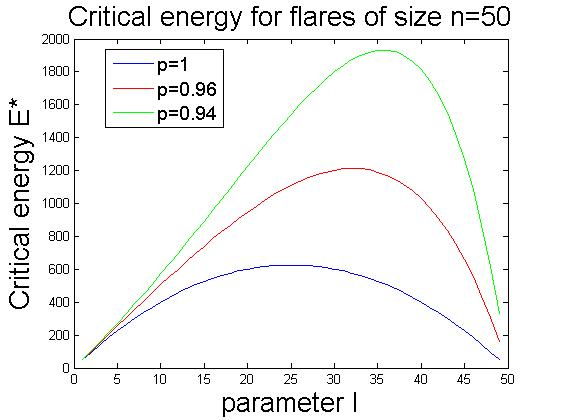
\includegraphics[width=0.8\textwidth]{flares.jpg}
    \caption{Plots of first critical energy for flares of size $n=50$ with respect to prameter $l$, $c=1,p=1,0.96,0.94$}
    \label{fig3}
\end{figure}

\begin{figure}[p]
    \centering
    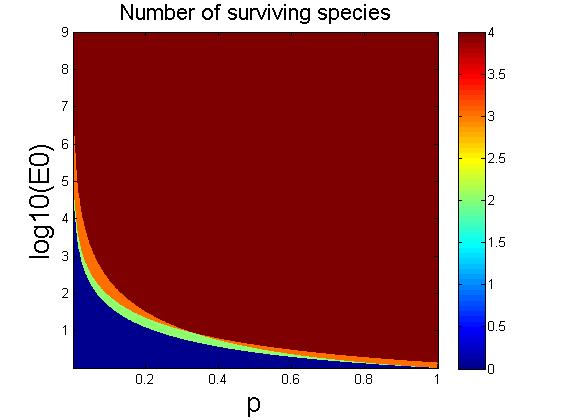
\includegraphics[width=0.8\textwidth]{4top5nodes.jpg}
    \caption{Number of surviving species for 4 topologies of size 5}
    \label{fig4}
\end{figure}

\begin{figure}[p]
    \centering
    
\includegraphics[width=0.8\textwidth]{untitled.jpg}
    \caption{minimized topologies}
    \label{fig5}
\end{figure}

\begin{figure}[p]
    \centering
    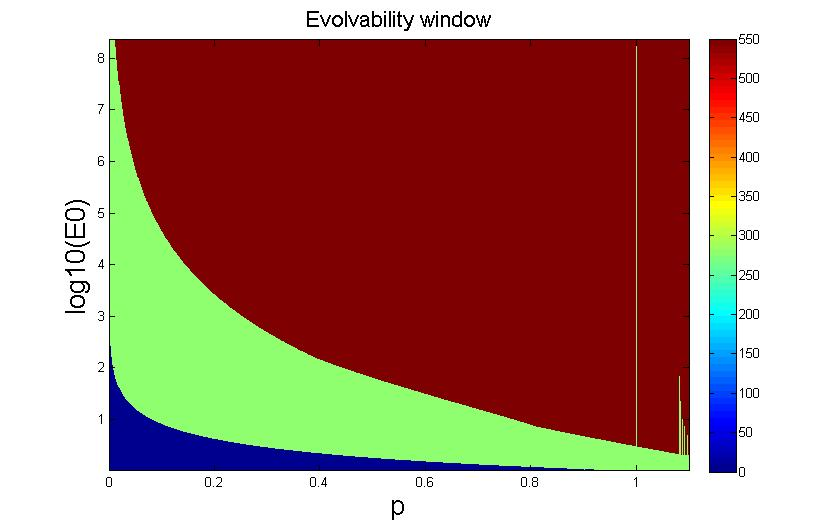
\includegraphics[width=0.8\textwidth]{topcycle.jpg}
    \caption{colormap of topologies with cycle and p>1}
    \label{fig6}
\end{figure}

\begin{figure}[p]
    \centering
    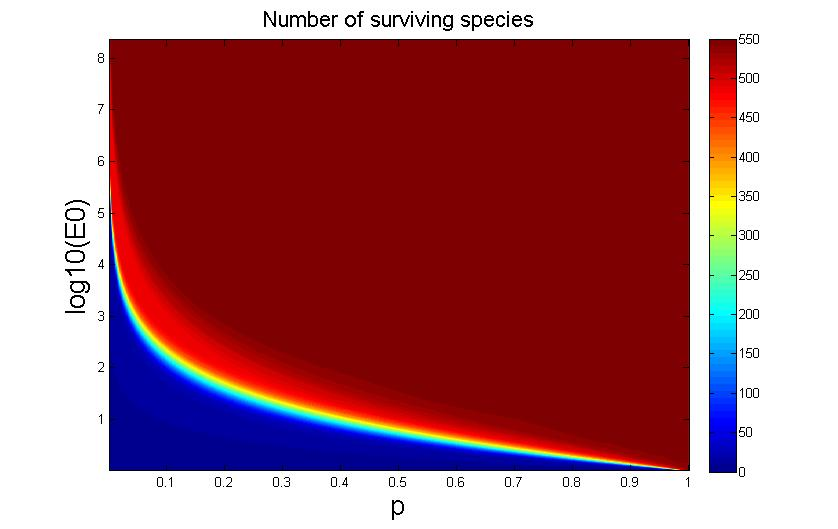
\includegraphics[width=0.8\textwidth]{colormap.jpg}
    \caption{Surviving topologies. Sizes $n=5,..,15$,with 50 each, random topologies}
    \label{fig7}
\end{figure}

\begin{figure}[p]
    \centering
    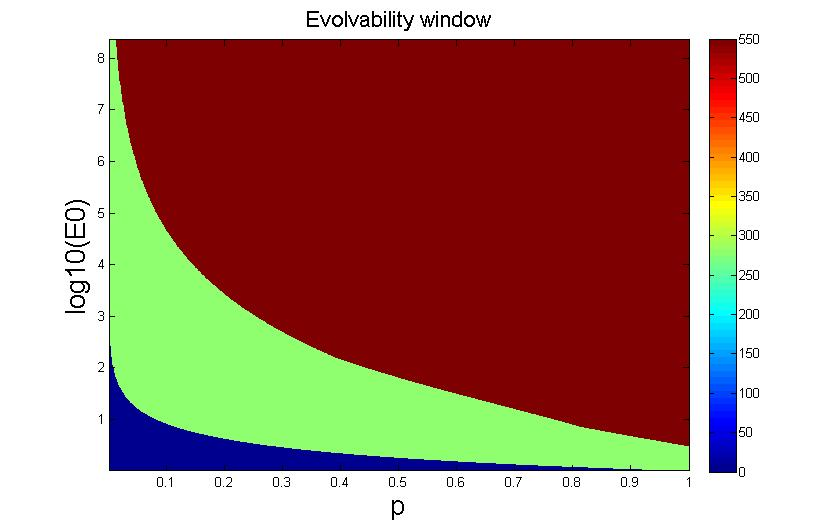
\includegraphics[width=0.8\textwidth]{evowind.jpg}
    \caption{Window of evolvability}
    \label{fig8}
\end{figure}

\begin{figure}[p]
    \centering
    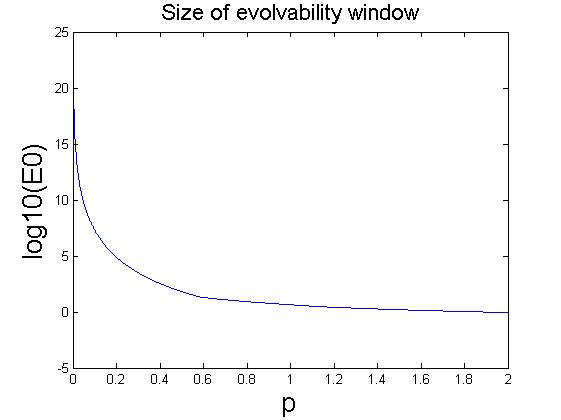
\includegraphics[width=0.8\textwidth]{sizeevo.jpg}
    \caption{size of window of evolvability for $0\leq p\leq 2$ no cycles $n=2,..10$, with total 3741 topologies (builder)}
    \label{fig9}
\end{figure}

\begin{figure}[p]
    \centering
    
\includegraphics[width=0.8\textwidth]{untitled.jpg}
    \caption{size of window of evolvability for $0\leq p\leq 2$ size $n=10$. (to redo)}
    \label{fig10}
\end{figure}

\begin{figure}[p]
    \centering
    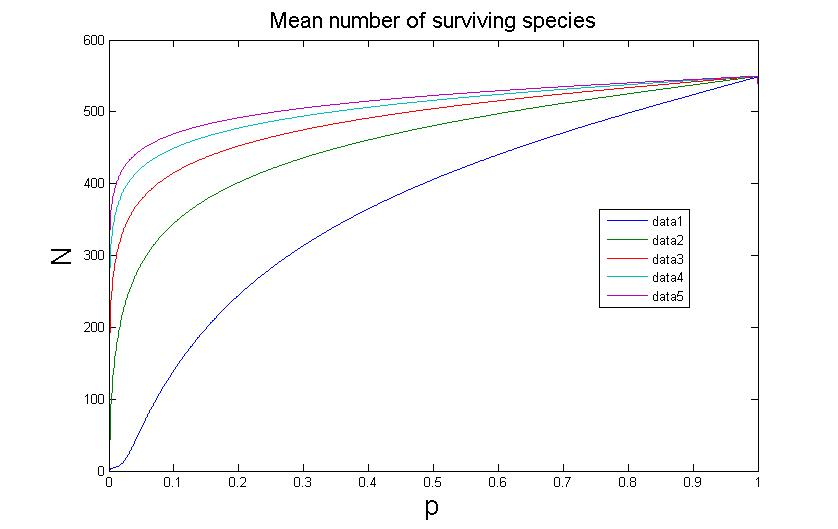
\includegraphics[width=0.8\textwidth]{means.jpg}
    \caption{mean number of surviving species for different mean energies (lowest to highest), as a function of $p$. Sizes $n=5,..,15$,with 50 each, random topologies }
    \label{fig11}
\end{figure}

\begin{figure}[p]
    \centering
    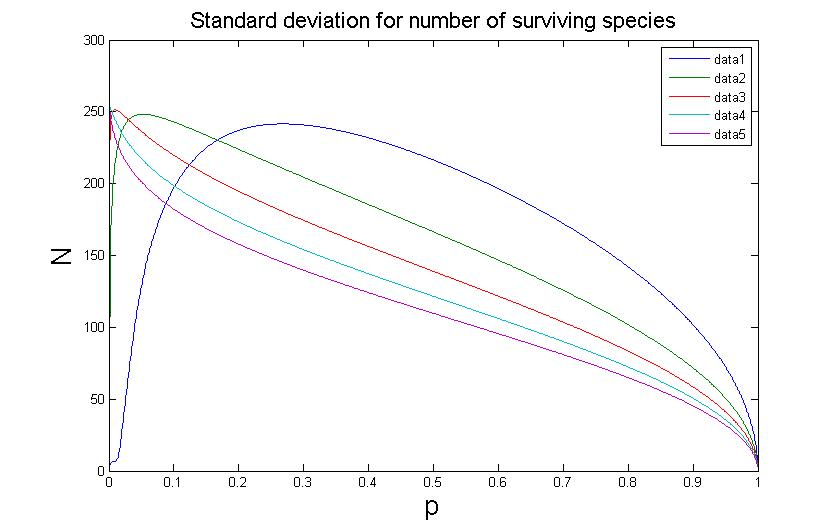
\includegraphics[width=0.8\textwidth]{std.jpg}
    \caption{standard deviation of number of surviving species for different mean energies (lowest to highest), as a function of $p$. Sizes $n=5,..,15$,with 50 each, random topologies}
    \label{fig12}
\end{figure}

\end{document}